\documentclass[11pt]{article}
\usepackage{fullpage}
\usepackage{listings}
\usepackage{needspace}
\usepackage{color}
\usepackage{ifthen}
\usepackage{pgf}
\usepackage{tikz}
\usetikzlibrary{arrows,automata}
\usepackage{amsmath}
\usepackage{url}
\usepackage{framed}
\usepackage{enumerate}
\usepackage{csc}
\usepackage{textcomp}
\usepackage{tabu}
\lstset{ %
basicstyle=\footnotesize\ttfamily,       % the size of the fonts that are used for the code
numbers=left,                   % where to put the line-numbers
stepnumber=1,                   % the step between two line-numbers. If it's 1 each line will be numbered
numbersep=5pt,                  % how far the line-numbers are from the code
showspaces=false,               % show spaces adding particular underscores
showstringspaces=false,         % underline spaces within strings
tabsize=4,		                % sets default tabsize to 4 spaces
language=Java,
upquote=true,
columns=fixed
}

\ifthenelse{\isundefined{\isAnswerKey}}
{
    \newenvironment{answer}{\large\lstset{basicstyle=\tiny\ttfamily}\color{white}}{}
}
{
    \newenvironment{answer}{\large\lstset{basicstyle=\footnotesize\ttfamily}\color{red}}{}
}


\author{Computer Science Community}
\title{CS-142 Final Exam Review}
\date{\today}

\makeatletter
\let\thetitle\@title
\let\theauthor\@author
\let\thedate\@date
\makeatother

\begin{document}
\header

\begin{enumerate}
\item Suppose we are talking about the depth-first search (DFS) algorithm. Nodes are added to the data structures in alphabetical order.
\begin{enumerate}
\item What underlying data structure does this algorithm use?

\begin{answer}
A stack.
\end{answer}

\item
Given the following graph, state the DFS traversal order and show the data structure at each step.
Node \texttt{A} is the start node, and \texttt{F} is the destination node.

\begin{minipage}{0.35\textwidth}
\vspace{-136pt}
\begin{answer}
$\leftarrow$ bottom of stack \\
\textbar A \\
\textbar B C \\
\textbar B D E \\
\textbar B D \\
\textbar B F \\
\textbar B \\

The traversal order is ACEDF.
\end{answer}
\end{minipage}
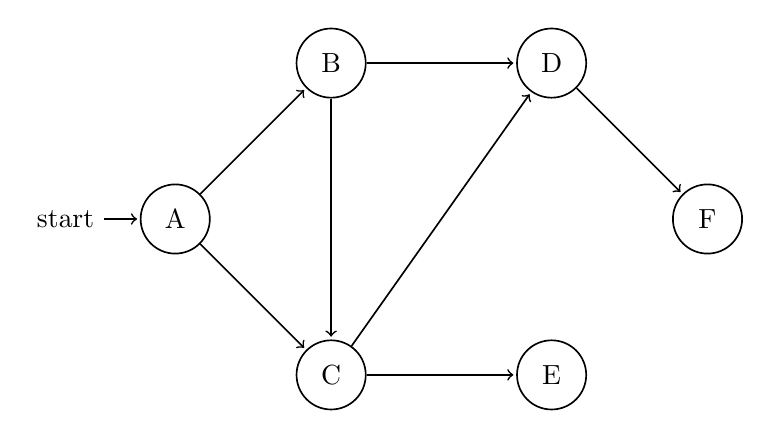
\begin{tikzpicture}[shorten >=1pt,auto,node distance=2.8cm,semithick]
	\node[initial,state] (A) {A};
	\node[state]        (B) [above right of=A] {B};
	\node[state]        (C) [below right of=A] {C};
	\node[state]        (D) [right of=B] {D};
	\node[state]        (E) [right of=C] {E};
	\node[state]        (F) [below right of=D] {F};

	\path[->]   (A) edge node {} (C)
		(A) edge node {} (B)
		(B) edge node {} (C)
		(B) edge node {} (D)
		(C) edge node {} (D)
		(C) edge node {} (E)
		(D) edge node {} (F);
\end{tikzpicture}

\item
What path from \texttt{A} to \texttt{F} does the DFS algorithm return?

\begin{answer}
ACDF 
\end{answer}

\end{enumerate}


\item Now consider a BFS algorithm, again populating data structures in alphabetical order.
\begin{enumerate}
\item
What changes would need to be made to a DFS implementation to turn it into a breadth-first search (BFS)?

\begin{answer}
Use a queue data structure (instead of a stack).
\end{answer}

\item
Using the graph as described in Question 1, what is the BFS traversal order?
Show the data structure at each step. \\
\begin{answer}
$\leftarrow$ front of queue \\
A \\
B C \\
C D \\
D E \\
E F \\
F \\

The traversal order is ABCDEF.
\end{answer}

\item
What path from \texttt{A} to \texttt{F} results from the BFS algorithm?

\begin{answer}
ABDF
\end{answer}

\end{enumerate}

\newpage
\item Which layout manager does each of the following descriptions describe?
\begin{enumerate}[(a)]

\item Displays the contained components in a set number of rows and columns,
      where each row has the same height and each column the same width.
\begin{answer}
GridLayout
\end{answer}

\vspace{6pt}
\item Attempts to display the contained components in a single row but will
      create a new row if necessary.
\begin{answer}
FlowLayout
\end{answer}

\vspace{6pt}
\item Allows the developer to specify the region (North, South, East, West,
      Center) of the panel to place the component in.
\begin{answer}
BorderLayout
\end{answer}

\end{enumerate}

\item Rick owns a positively popular pizza place conveniently located just off of campus.
	Originally, he made all the pizzas himself, but rising campus food prices are making demand skyrocket.
	Luckily, the college students are as desperate for money as they are for food, a situation from which Rick, being a pragmatic individual, finds he can benefit.
	Drawing from the exploitable labor pool, Rick turns his already-hot kitchen into a sweat shop, ordering his workers like so:
	\begin{lstlisting}[numbers=none]
	for ( PizzaSlave student : laborPool ) {
		new Thread(student) . run();
	}
	\end{lstlisting}
	Sensing an early retirement, Rick promotes his first hire from slave to manager, rewarding him with slightly higher---but still illegal---pay.
	(Despite these perks and the envy of his peers, the manager is just like everyone else.)
	Alas, when Rick returns a few days later, he is so displeased with what he sees that he fires the manager on the spot.
	What made Rick so angry, and what should he have done differently to prevent its happening?

	\begin{answer}
	In his haste to make a profit, Rick mistakenly called the \texttt{Thread} class's \texttt{run()} method, which caused his manager to run synchronously and make pizzas while everyone else stood around waiting.
	Rick should instead have called \texttt{start()}, which would have whipped all of his workers into shape at roughly the same time.
	\end{answer}

\item {\bf The Life of Nick:}
    Nick, an aspiring entrepreneur, trained for 7 grueling years in the jungles of Zimbabwe.
    Nick's preparation was overseen by a group of trainers. His stages of learning were
    fueled by the following process:
    \begin{lstlisting}[numbers=none]
    public class Nick {
        private int experience = 0 ;
        public void train ( ) {
            this.experience += 1 ;
        }
    }\end{lstlisting}Imagine instructors are threads in Java. What are some problems
    we may encounter if Nick is having multiple people train him at the same time?
    How might we remedy these issues?

    \begin{answer}
    The train function, and specifically its incrementation, is non-atomic, meaning the value of Nick's 
    \texttt{experience} variable will be undefined after multiple threads attempt to call the function concurrently.  One solution would be to synchronize on \texttt{Nick} to ensure only one thread at a time executes within the critical section.\\
    \end{answer}

\pagebreak
\item {\bf Nick's Heavy Threads:}
	Nick now operates a store in Marketview Mall which
      has poor lighting, blasts black metal and sells jeans. Only one pair of
      jeans is available to purchase at a time, though there are more
      stored in the back. If a size is out that you don't want, you must wait
      for someone else to purchase the jeans. Nick's only employee, Hank, sits
      in a chair and stares at people angrily until someone makes a purchase,
      at which point he replaces the jeans with the same model of a random
      size. In order to prevent customers' waiting infinitely for an
      unavailable size, Hank will switch the jeans for a different size pair if
      no one has bought them after a period of three seconds.

\begin{lstlisting}
public class NicksHeavyThreads
{
	// jeans' size [1-5], or 0 when none on display
    private static int awesomeJeans = 0;
    
	// keep this updated as customers arrive and leave
    private static int customers = 0;
    
    private static MeanWorker hank = new MeanWorker();
    
    public static void main( String[] args )
    {
        for( int i = 0; i < 10; ++i )
        {
            ( new LameCustomer() ).start();
        }

		// wait one second before introducing Hank
        try { Thread.sleep( 1000 ); }
        catch( InterruptedException pleaseDont ) {}
        hank.start();
    }
    
    private static class LameCustomer extends Thread
    {
        // ( implementation omitted )
    }
    
    private static class MeanWorker extends Thread
    {
        // ( implementation omitted )
    }
}
\end{lstlisting}
\scriptsize
(Questions may be found on the next page. You may answer them in the space allotted here, or on the following page.)
\normalsize

    \begin{enumerate}

	\pagebreak

    \item Complete the implementation of the \texttt{LameCustomer} class: Each instance
          must choose a jeans size and wait for it to be available, update the
          jeans to indicate that they have been taken, print the message
          ``Customer: I got my size \emph{size} jeans!" and inform all threads
          that the jeans selection has changed. \\
		  \textit{(Hint: Remember to keep an
          accurate count of how many customers are in the shop.)}

\begin{answer}
\begin{lstlisting}
static class LameCustomer extends Thread {
    public void run() {
        synchronized( hank ) {
            ++customers;
			// pick size
            int desiredSize = (int) ( Math.random()*(5) ) + 1;
			// wait for pair
            while( awesomeJeans != desiredSize ) {
                try { hank.wait(); }
                catch( InterruptedException pleaseDont ) {}
            }
            System.out.println( "Customer: I got my size "
                + awesomeJeans + " jeans!" );
            awesomeJeans = 0; // take the jeans
            hank.notifyAll(); // inform everyone they are gone
            --customers;
        }
    }
}
\end{lstlisting}
\end{answer}

    \item Now implement the \texttt{MeanWorker} class, which should choose a size and
          stock a pair of jeans of that size, print the message ``Hank: I
          grumpily restocked with size \emph{size}," and inform all threads
          that the selection has changed. It should then wait until someone has
          taken the jeans or until three seconds have elapsed, whichever comes
          first. These steps should be repeated until all customers have left
          the store.

\begin{answer}
\begin{lstlisting}
static class MeanWorker extends Thread {
    public synchronized void run() {
        do {
			// new size
            awesomeJeans = (int) ( Math.random()*(5) ) + 1;
            System.out.println( "Hank: I grumpily restocked "
                + "with jeans of size " + awesomeJeans );
            notifyAll(); // inform customers of the restocking
            try { wait( 3000 ); } // let people shop
            catch( InterruptedException pleaseDont ) {}
        }
        while( customers > 0 );
    }
}
\end{lstlisting}
\end{answer}
    \end{enumerate}

\pagebreak
\item Briefly describe the difference (for objects) between \texttt{a.equals(b)}, \texttt{a==b}, \texttt{a.compareTo(b)},\\ and \texttt{Comparator.compare(a,b)}.

\begin{answer}
\begin{itemize}

\item \texttt{a.equals(b)} Compares objects for equality. 
Class \texttt{Object} provides a default implementation (to be precise, it is \texttt{==} by default) that can be overridden for behavior necessary for a certain class. Returns a \texttt{boolean}.

\item \texttt{a == b}  Checks \textit{memory locations} (if the two objects are the SAME object, as defined by whether or not \texttt{a} and \texttt{b} point to the same spot in memory). Can also be used to check whether \texttt{a} is \texttt{null}. Also returns a \texttt{boolean}.

\item \texttt{a.compareTo(b)} Returns an \texttt{int} indicating whether \texttt{a} is less than (-1),
equal to (0), or greater than (+1) \texttt{b}, according to their natural ordering. Specified by the \texttt{Comparable} interface.

\item \texttt{compare(a,b)} Returns a negative a $<$ b, 0 if a $=$ b, a positive if a $>$ b. \\
With two \texttt{Comparator} objects, \texttt{comp1} and \texttt{comp2},
\texttt{comp1.equals(comp2)} implies that \\ \texttt{sgn(comp1.compare(o1,o2))==sgn(comp2.compare(o1, o2))} for every object reference \texttt{o1} and \texttt{o2}.

\end{itemize}
\end{answer}


\pagebreak
	\item Consider the following graph. \\
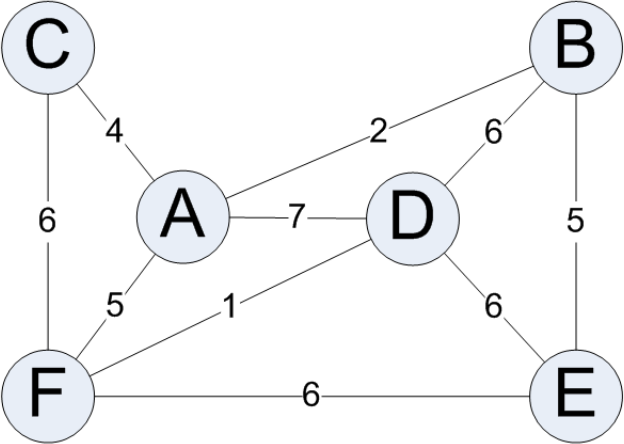
\includegraphics[height=150px]{other/graph.png}
\begin{enumerate}
	\item
	Perform Dijkstra's algorithm to find the shortest path between C and E. \\
	\def\arraystretch{1.65}
	\begin{tabu}{| c | c | c | c | c | c | c |}
		\hline
		Finalized & A & B & C & D & E & F\\
		\hline
		-- & ($\infty$, None) & ($\infty$, None) & \textbf{(0, None)} & ($\infty$, None) & ($\infty$, None) & ($\infty$, None) \\
		\answerrow{C & \textbf{(4, C)} & ($\infty$, None) & (0, None) & ($\infty$, None) & ($\infty$, None) & \textbf{(6, C)}} \\
		\answerrow{A & (4, C) & \textbf{(6, A)} & (0, None) & \textbf{(11, A)} & ($\infty$, None) & (6, C)} \\
		\answerrow{F & (4, C) & (6, A) & (0, None) & \textbf{(7, F)} & \textbf{(12, F)} & (6, C)} \\
		\answerrow{B & (4, C) & (6, A) & (0, None) & (7, F) & \textbf{(11, B)} & (6, C)} \\
		\answerrow{D & (4, C) & (6, A) & (0, None) & (7, F) & (11, B) & (6, C)} \\
		\answerrow{E & (4, C) & (6, A) & (0, None) & (7, F) & (11, B) & (6, C)} \\
		\hline
	\end{tabu} \\

	\begin{answer}
		The shortest path is CABE with a total cost of 11.
		To reconstruct this solution, we start with the destination node, then move on to its recorded optimal predecessor.
		We repeat the process until we reach the starting node.
		(Note that this isn't the only possible table.)
	\end{answer}

	\item
	In general, when using Dijkstra's algorithm to find the shortest path between nodes,
	do you need to use every row of the table? Why or why not?

	\begin{answer}
		No. The algorithm is finished as soon as the destination node has been finalized;
		Dijkstra's is a greedy algorithm so it will never change decisions once they are made.
	\end{answer}
\end{enumerate}

	\item Why does Dijkstra's algorithm not work correctly on graphs with negative
      edge weights?

\begin{answer}
Dijkstra's algorithm doesn't work correctly on graphs with negative edge
weights due to one of its {\em greedy} behaviors.

When selecting the next node to visit, Dijkstra's algorithm chooses the
node with the current lowest total value, then {\em finalizes} that value
forever. If there were another route to that node, which had not yet been
explored (and contained a net negative weight) Dijkstra's algorithm would
return a suboptimal path.
\end{answer}


\vspace{24pt}
	\item What role does the priority queue play in finding the shortest path?
      When do we use it?

    \begin{answer}
    The priority queue is used to select the next vertex to visit. We want to
    visit the node which currently has the lowest tentative distance from the
    start, so we use a priority queue that always returns the lowest element.
    \end{answer}
	\item When is a vertex's sum weight finalized in Dijkstra's algorithm?

    \begin{answer}
    A vertex's sum weight is final after it has updated the tentative distances
    of all of its neighbors. As part of being finalized, it's moved from the
    unvisited set to the visited set.
    \end{answer}

\pagebreak
\item Assume the following line of code is given:
\begin{lstlisting}[numbers=none]
	Collection<Integer> t = new ArrayList<Integer>();
\end{lstlisting}

What then is wrong with the following? Correct any errors:
\begin{lstlisting}[numbers=none]
	for( int i = 0; i < 20; ++i ){
		t.add(i);
       }
       for( int i=0; i <  t.size(); ++i ){
		System.out.println(t.get(i));
       }
\end{lstlisting}

\begin{answer}
\texttt{Collection} does not support \texttt{get(i)}. The better solution is:
\begin{lstlisting}[numbers=none]
	for( int i = 0; i < 20; ++i ) {
		t.add(i);
       }
       for( Integer i : t ) {
		System.out.println(i);
       }
\end{lstlisting}
\end{answer}


\item Briefly explain the differences between the three kinds of exceptions: checked exceptions, runtime exceptions, and errors.
\begin{answer}

\textbf{checked exceptions} -� Exceptions that a method signature must specify it throws. If a method
may throw a checked exception, all calls to that method must be within a \texttt{try}-\texttt{catch} block. Checked exceptions should be used exclusively for foreseeable runtime mistakes, and any reasonably robust
system should be able to recover from one. Classic example is \texttt{IOException}.\\

\textbf{runtime exception} -� Not declared in a method signature and not anticipated to be thrown.
Usually arise due to software bugs and often cause the program to crash. Classic
examples are \texttt{NullPointerException} and \texttt{ArrayIndexOutOfBoundsException}.\\

\textbf{errors} -� Represent a serious issue outside of the control of the programmer (hard drive
failure, not enough memory, device issue). Examples are \texttt{IOError}, \texttt{VirtualMachineError} and
\texttt{ThreadDeath} (see Java's \texttt{Error} class).
\end{answer}


\vspace{48pt}

\pagebreak
\item Use the following code to answer the questions listed on the next page.

\lstinputlisting{other/code/ufo/UFO.java}

\pagebreak
\begin{enumerate}
\item Why should \texttt{Probable} be an interface, rather than a class or an abstract class?

\begin{answer}
\texttt{Probable} needs to define that certain actions can be performed on \texttt{Probable} objects, but does not need to define what those actions should do.
\end{answer}

\item Write the \texttt{Probable} interface.

\begin{answer}
\lstinputlisting{other/code/ufo/Probable.java}
\end{answer}

\item Should the \texttt{Redneck} and \texttt{Professor} classes implement \texttt{Probable} directly?

\begin{answer}
No! Since \texttt{Redneck} and \texttt{Professor} objects are stored in variables of type \texttt{Human}, they must extend the \texttt{Human} class.
In addition, since the \texttt{Human} variables are able to be added into a collection of \texttt{Probable} objects, the \texttt{Human} class must implement \texttt{Probable}, which will carry down into the \texttt{Redneck} and \texttt{Professor} classes.
\end{answer}

\end{enumerate}

\item \textbf{Networking} 
	\begin{enumerate}
		\item What does TCP stand for? Where and why do we use TCP?
		
		\begin{answer}
		TCP stands for Transmission Control Protocol. We use TCP in Telephone Connection because TCP guarantees packet delivery and thus can be considered "lossless and reliable".
		\end{answer}
		
		\item What does UDP stand for? When and where do we use UDP?
		
		\begin{answer}
		User Datagram Protocol. We use UDP when we are managing a tremendous amount of state (ex: weather data, video transmission).
		\end{answer}
		
		\item Which one does a stream socket use for data transmission? TCP (or) UDP?
		
		\begin{answer}
		TCP. 
		\end{answer}
		
		\item Which one does a datagram socket use for data transmission? TCP (or) UDP?
		
		\begin{answer}
		UDP.
		\end{answer}
		
		\item What is a datagram?
		
		\begin{answer}
		A datagram is an independent, self-contained message sent over the network with no guarantees. % TODO: wording?
		\end{answer}
		
		\item What is a socket?
		
		\begin{answer}
		A socket refers to the endpoints of logical connections between two hosts, which can be used to send and receive data.
		\end{answer}
	
	\end{enumerate}

\newpage
\item Find at least 3 (total) errors in the following code:

	\textit{Server: echoes one line of data sent to it}
\begin{lstlisting}
	ServerSocket pubServer = new ServerSocket(0);
	System.out.println(pubServer.getLocalPort());
	Socket client;
	BufferedReader reader = null;
	try {
		reader = new BufferedReader(
			new InputStreamReader(client.getInputStream()));
	} catch (IOException e) {
		System.out.println("IOException: " + e.getMessage());
	}
	String response = null;
	try {
		response = reader.readLine();
	} catch (IOException e) {
		System.out.println("IOException: " + e.getMessage());
	}
	System.out.println(response);
	pubServer.close();
\end{lstlisting}

	\textit{Client: sends a line of text to a server: server address, port, text}
\begin{lstlisting}
	InetAddress server = null;
	try {
		server = InetAddress.getByName(args[0]);
	} catch (UnknownHostException e) {
		System.out.println("Unknown host");
	}
	int port = Integer.parseInt(args[1]);
	Socket conn = null;
	try {
		conn = new Socket(server, port);
	} catch (IOException e) {
		System.out.println("IOException: " + e.getMessage());
	}
	try {
		System.out.println(args[2]);
	} catch (IOException e) {
		System.out.println("IOException: " + e.getMessage());
	}
	conn.close();
\end{lstlisting}
\begin{answer}
	\begin{enumerate}
	\item
		Server: reader is not always instantiated!
	\item
		Server: client never initialized, use pubServer.accept().
	\item
		Server: Missing client.close().
	\item
		Server and Client: *.close() should be in a try-catch block.
	\item
		Client: Need a PrintWriter writer; writer = new PrintWriter(conn.getOutputStream(), true); writer.println(args[2]); instead of System.out.println(args[2]);
	\end{enumerate}
\end{answer}


\newpage
\item Name the design pattern used in the following snippet of code.
\begin{lstlisting}
public class Car
{
	private String make;
	private String model;
	private int mileage;

	private Car(String make, String model, int mileage)
	{
		this.make=make;
		this.model=model;
		this.mileage=mileage;
	}
	public static Car makeCar(String str)
	{
		String arr[] = str.split(" ");
		return new Car(arr[0], arr[1], Integer.parseInteger(arr[2]));
	}

	public static void main(String[] args)
	{
		Car myCar = Car.makeCar("Toyota Camry 200000");
	}
}
\end{lstlisting}

\begin{answer}
The \emph{Factory} design pattern is used.
\vspace{.5in}
\end{answer}

\end{enumerate}

\end{document}
